\documentclass[12pt]{article}
\usepackage{graphicx}
\graphicspath{ {./images/} }
\usepackage{amsmath}
\usepackage[compact]{titlesec}
\usepackage{titling}
\usepackage{lmodern}
\usepackage[table]{xcolor}
\usepackage[top=2cm,left=2cm,right=2cm,bottom=2cm]{geometry}
\usepackage[caption=false,font=footnotesize]{subfig}
\usepackage{url}
\usepackage{hyperref}
\hypersetup{bookmarks,breaklinks,letterpaper,colorlinks,urlcolor=cyan,linkcolor=blue,filecolor=magenta,citecolor=black}
\usepackage{xspace}
\makeatletter
\newcommand*\bigcdot{\mathpalette\bigcdot@{.5}}
\newcommand*\bigcdot@[2]{\mathbin{\vcenter{\hbox{\scalebox{#2}{$\m@th#1\bullet$}}}}}
\makeatother
% \renewcommand\maketitlehookc{\vspace{-9ex}}
\usepackage{tabularray}
\newcommand{\sym}[1]{\textit{#1}}
\newcommand{\ie}{i\cdot e\cdot \xspace}
\newcommand{\eg}{e\cdot g\cdot \xspace}
\usepackage{multirow}
\newcolumntype{P}[1]{>{\centering\arraybackslash}p{#1}}
\begin{document}

\title{\vspace{-3cm}CS 335 Semester 2022--2023-II: Project Milestone }
\author{Dishay Mehta (200341) Shrey Mehta (200580) Shubhan R (200971)}
\date{\today}
\maketitle

\section*{}
README file:\\
The environment should have flex and bison installed.\\
If its Linux then it can be installed from the command "sudo apt install flex".\\
If its Linux then it can be installed from the command "sudo apt install bison".\\
The system should also have g++ installed.\\

\subsection*{Compilation and Execution}
Go to the required directory by command "cd src" \\
Enter "make" on the command line to build the src folder\\
We have created a wrapper code to make the milestone3\\
To execute,\\
Enter the command "cd /path/to/root"\\
Then the command "./milestone3 -i $<$inputfile$>$"\\
Note: You are required to change each and every file in rwx mode, i.e. do chmod 777 to each and every file in case of access denial.

\subsection*{Output}
We have the output generated in our terminal itself.\\
This output will be the 3ac code for the input java testcode.

\subsection*{Compile Instructions}
The following command line options have been implemented by us
\begin{itemize}
    \item -i : The input flag where the input file must be fed.
    \item -v : the verbose option which provides the debugging info in case of any errors in the code.
    \item -h : The help option which lists the execution instructions. 
\end{itemize}

\subsection*{Implementation Details}
% \subsubsection*{Symbol Table}
% \begin{itemize}
%     \item We have maintained two classes named Sym\_Entry and Sym\_Table, the first class storing the fields of the symbols and the Sym\_Table storing a map which is the symbol table, the parent pointer, which points to the parent of that scope of the symbol table, and the level number of that symbol table.
%     \item The symbol table which has scope named "Global" is the global scope of the file being parsed, and has level = 0 and parent pointing to NULL. 
%     \item The symbol table has fields: Lexeme, Token, Type, Offset, Scope Name and Line Number. The other fields which are present in the class were used for implementing specific functionalities. 
%     \item The corresponding semantic actions were added in each production, such that the scope is changed and a new symbol table is formed, each time we enter a new scope and the previous table is stored in a vector of symbol tables which can later be accessed by their scope names for type checking.
%     \end{itemize}
%     \subsubsection*{Type Checking}
%     We have run many experiments on real Java compilers to understand type checking rules to make sure our type checking rules agree with standards. We have also read many online websites regarding how classes and objects and static etc. work. We have done type checking for all expressions and operators, methods, arrays, classes. Even static, public, private and final type checking as specified on the forum are implemented. We have added appropriate error messages with the line numbers also. \textbf{System.out.println may give error in some code lines as this as not been implemented yet and the instructor has told us to ignore it on Piazza. Please consider the error due to this accordingly.}\\
%     We have also implemented type-casting as asked in the description of the milestone 2. 
    \subsubsection*{Three Address Code}
    \textbf{The final 3ac code is printed in the terminal. We have also dumped the files. In case any of the dump files are missing please consider the terminal one as final.} We have used Quadruple representation of the 3AC code in the implementation. A struct is made to store this and a vector of this struct is maintained and the 3AC code corresponding to each expression is pushed into this vector, which are  dumped in CSV files for each functions at the end.
    We have added the 3AC code corresponding to each and every function following the following format:
    \begin{itemize}
        \item Expressions: \\
        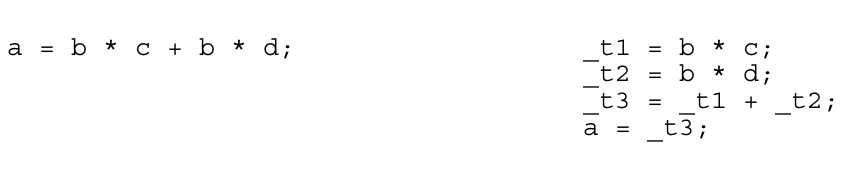
\includegraphics[scale = 0.4]{expr.png}
        \item Array Access: \\
        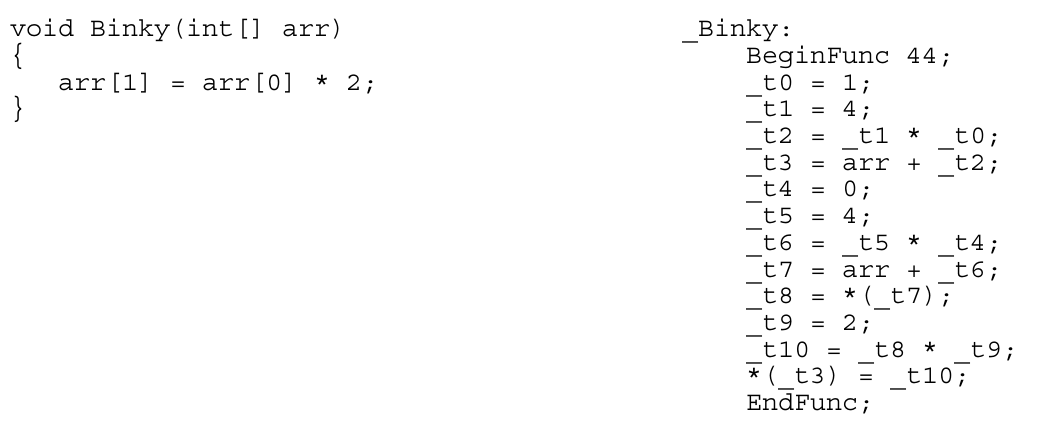
\includegraphics[scale = 0.4]{array.png}
        \item If-Else Statements \\
        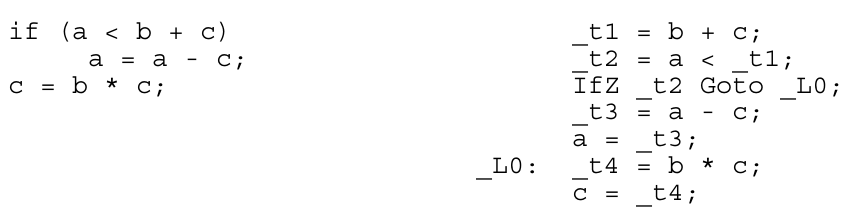
\includegraphics[scale = 0.4]{ifelse.png}
        \item Loops ( While loop shown, similarly for others ) \\
        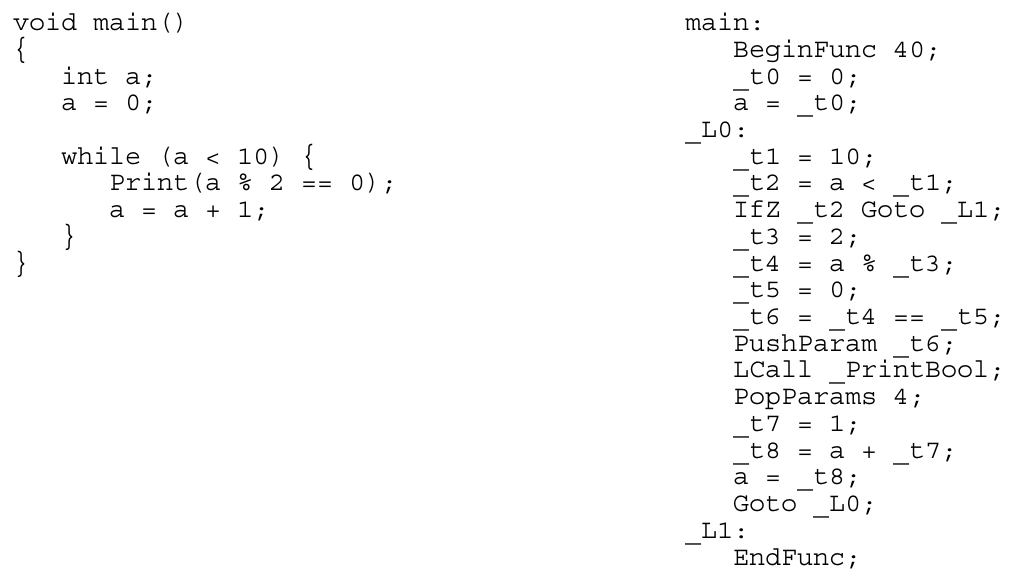
\includegraphics[scale = 0.4]{Loops.png}
        \item Method Invocation \\
        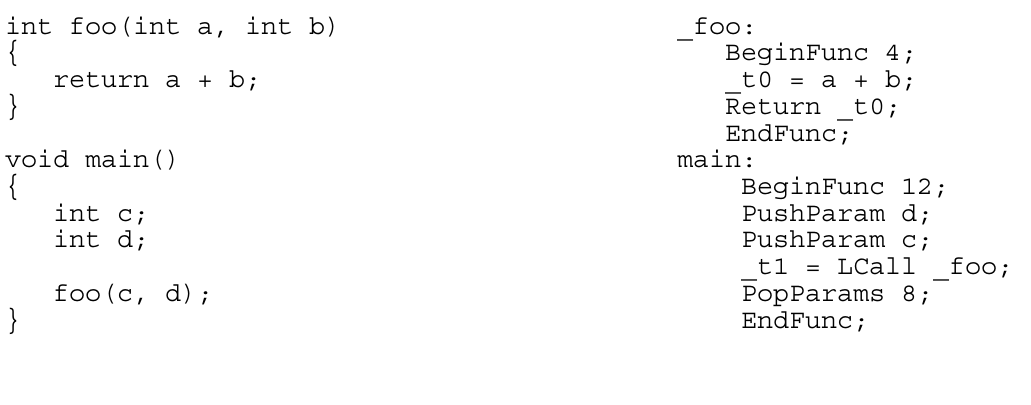
\includegraphics[scale = 0.4]{method.png}
        \item ClassInstanceCreation \\
        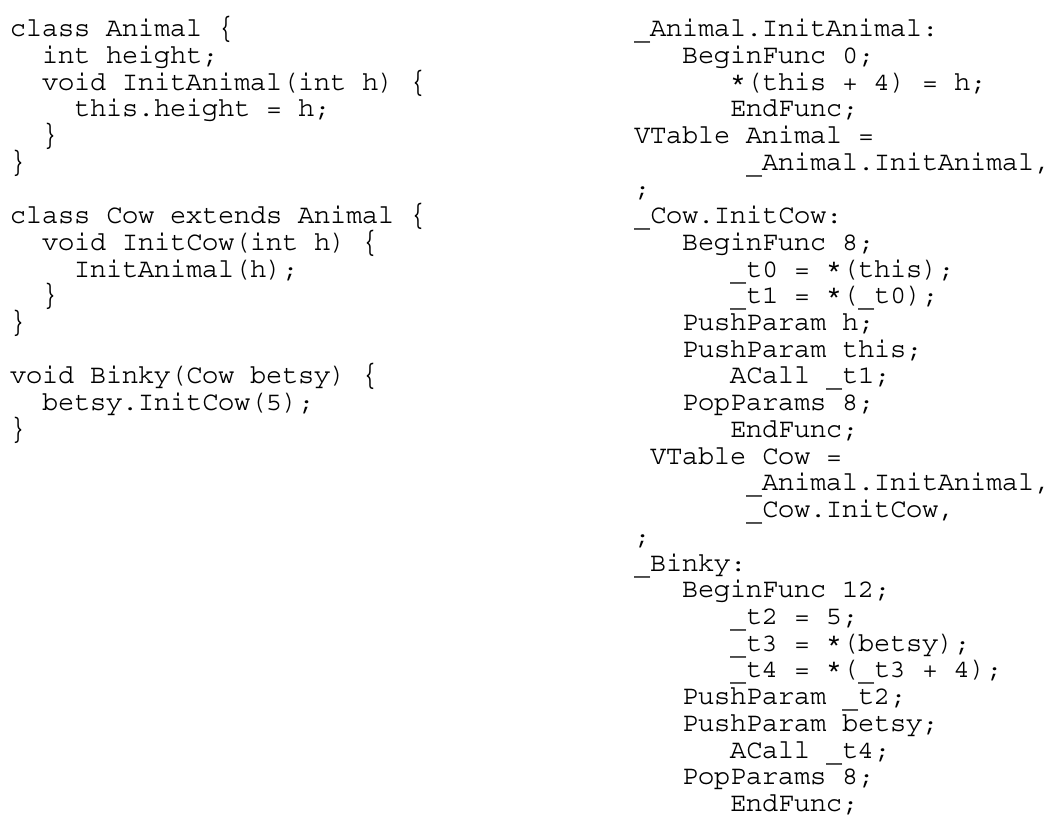
\includegraphics[scale = 0.4]{class.png}
    \end{itemize}
    Corresponding to these rules, the 3AC code has been made. Beginning of class and function have been indicated by BeginClass and BeginFunc respectively in the .3ac file.
    We have also implemented the cast\_to\_int etc.
    \newpage
    \subsection*{Stack}
    To showcase our implementation of stack, let us take an example of a very simple function code:\\\\
    int f(int a,int b)\\ \{ \\
    \hspace*{5mm}int x;\\
    \hspace*{5mm}return a;\\ \}
 
\begin{table}[h]
\caption{Downward Growing Stack}
\centering
\begin{tabular}{|P{3cm}|}
\hline
b \\ \hline
a \\ \hline
RA \\ \hline
BP \\ \hline
x \\ \hline
\big\downarrow \\ \hline
\end{tabular}
\end{table}
    
    \subsection*{Assumptions}
    \begin{itemize}
        \item We have assumed that only the types present in raw JAVA language are allowed. The types like "String" are not supported by us.
        \item We have throwing errors for the basic type-checking errors which are the static compilation checks done while parsing the grammar.
        \item The Three AC code has been made according to the rules above, which is a different representation as compared to the example given on piazza ( This 3AC encoding is a reference from Handout written by Maggie Johnson and revised by Julie Zelenski )
        \item We have added support to access modifiers like public, private, static and final only just as mentioned on Piazza.
        \item We have not given errors for the variables which are assigned without initialisation, as that is a compiler developer dependent property, as has been mentioned in the JAVA Documentation.
        \item Kindly ignore any errors due to System.out.println() in the 3AC Code.
        \item All the basic features as mentioned on Piazza have been incorporated in the submission.
        \item Even if the file may be erroneous, the symbol table dumps and the 3AC code will be generated.
        \item Kindly ensure that the class names don't start with string "Class" and Methods don't start with "Method" for dumping purposes.
        \item All the functions must be declared before used, i.e. you cannot call a function defined later before calling it as we wanted to generate all the specified functionalities in one parse through the input string. If required, we may perform 2 parses, in which in the first parse, we make the symbol table and in the second parse, we can do the typechecking and generate the Three AC Code.
        \item  The arrays which are allocated using new are allocated in the heap memory, so they do not have any offset, since their dimensions may be variable and hence are defined in dynamic memory and not static memory.
    \end{itemize}

\subsection*{References}
\href{http://web.archive.org/web/20151010192637/http://www.dound.com/courses/cs143/handouts/17-TAC-Examples.pdf}{Handbook written by Maggie Johnson and revised by Julie Zelenski} \\
\href{https://web.stanford.edu/class/archive/cs/cs143/cs143.1128/lectures/13/Slides13.pdf}{Stanford Compiler Design Lecture 13}

\end{document}
